\documentclass[12pt,a4paper]{report}
\usepackage[utf8]{inputenc}
\usepackage{float}
\usepackage{times}
\usepackage{latexsym}
\usepackage{url}
\usepackage{savetrees}
\usepackage{apacite}
\usepackage{natbib}
\usepackage{graphicx}
\usepackage[caption = false]{subfig}
\usepackage{pgfplots}
\usepackage{pgfplotstable}
\usepackage{xspace}
\usepackage{xcolor}
\usepackage{paralist}
\usepackage{amsmath}
\usepackage{booktabs}
\usepackage{siunitx}
\usetikzlibrary{angles, arrows.meta, quotes}
\usepackage{relsize}
\usepackage{etoolbox}
\usepackage{enumerate}
\graphicspath{ {Figures/} }
\renewcommand{\baselinestretch}{1.5}
\usepackage[left=1in,right=1in,top=1in,bottom=1in]{geometry}
% argument #1: any options
%% local settings
\sisetup{detect-weight,mode=text}
% for avoiding siunitx using bold extended
\renewrobustcmd{\bfseries}{\fontseries{b}\selectfont}
\renewrobustcmd{\boldmath}{}
% abbreviation
\newrobustcmd{\B}{\bfseries}
% shorten the intercolumn spaces
\addtolength{\tabcolsep}{-4.1pt}
\pgfplotstableread{
x   farahm  reddy   ramisch discoj
doc2vec .088  .025 .039    .003 
Infersent   .019    .527    .221    .202
fastText    .295    .285    .446    .353
ELMo    .283    .406    .486   .316
BERT    .193    .372    .107    .181
Flair   .23 .102   .311    .303
word2vec    .35 .634    .581    .427
}\datasetq
\pgfplotstableread{
x   direct para combined
doc2vec .039    .388    .419
Infersent   .221    .712    .712
fastText    .446    .703    .703
ELMo    .459    .546    .546
BERT    .086    .583    .583
Flair   .295    .492    .492
word2vec    .581    .510    .677
}\datasetp
\newcommand{\embmethod}[2][]{\textsf{#2}$_{\text{#1}}$\xspace}
\newcommand{\wordtovec}{\embmethod{word2vec}}
\newcommand{\infersent}[1][]{\embmethod[#1]{infersent}}
\newcommand{\doctovec}{\embmethod{doc2vec}}
\newcommand{\elmo}{\embmethod{ELMo}}
\newcommand{\elmocon}{\embmethod{ELMo\textsubscript{context}}}
\newcommand{\fasttext}{\embmethod{fastText}}
\newcommand{\fasttextpre}{\embmethod{fastText\textsubscript{pre}}}
\newcommand{\glove}{\embmethod{GloVe}}
\newcommand{\bert}{\embmethod{BERT}}
\newcommand{\bertcon}{\embmethod{BERT\textsubscript{context}}}
\newcommand{\flair}{\embmethod{Flair}}
\newcommand{\flaircon}{\embmethod{Flair\textsubscript{context}}}

\newcommand{\dataset}[2][]{\textsc{#2}$_{\text{#1}}$\xspace}
\newcommand{\reddy}{\dataset{Reddy}}
\newcommand{\ramisch}{\dataset{Ramisch}}
\newcommand{\discoj}[1][]{\dataset[#1]{DiSCo}}
\newcommand{\farahm}{\dataset{Farahmand}}

\newcommand{\method}[2][]{\ensuremath{\text{#2}_{\text{#1}}}\xspace}
\newcommand{\presum}{\method[pre]{Direct}}
\newcommand{\postsum}{\method[post]{Direct}}
\newcommand{\firstpara}{\method{Para\_first}}
\newcommand{\avgparapre}{\method[pre]{Para\_all}}
\newcommand{\avgparapost}{\method[post]{Para\_all}}
\newcommand{\combined}{\method{Combined}}

\newcommand{\MWEvec}{\ensuremath{\mathbf{mwe}}\xspace}
\newcommand{\paravec}[1][]{\ensuremath{\mathbf{para_{#1}}}\xspace}
\newcommand{\MWEonevec}{\ensuremath{\mathbf{w_1}}\xspace}
\newcommand{\MWEtwovec}{\ensuremath{\mathbf{w_2}}\xspace}

\newcommand{\tabref}[2][]{Table#1~\ref{#2}\xspace}
\newcommand{\figref}[2][]{Figure#1~\ref{#2}\xspace}
\newcommand{\secref}[2][]{Section#1~\ref{#2}\xspace}

\begin{filecontents}{alpha_reddy.dat}
X	elmo	bert	fasttext	w2v	d2v	is1	is2	flair
0.0	0.278	0.332	0.252	0.463	0.025	0.329	0.312	0.024
0.1	0.311	0.345	0.266	0.496	0.023	0.369	0.349	0.003
0.2	0.344	0.352	0.278	0.531	0.019	0.412	0.391	-0.021
0.3	0.375	0.349	0.285	0.563	0.013	0.454	0.437	-0.050
0.4	0.397	0.335	0.285	0.591	0.006	0.487	0.482	-0.081
0.5	0.406	0.311	0.274	0.611	-0.004	0.500	0.516	-0.113
0.6	0.399	0.281	0.255	0.622	-0.015	0.487	0.527	-0.143
0.7	0.381	0.249	0.228	0.620	-0.023	0.453	0.511	-0.167
0.8	0.355	0.218	0.200	0.608	-0.030	0.409	0.474	-0.184
0.9	0.328	0.189	0.172	0.587	-0.033	0.364	0.427	-0.195
1.0	0.301	0.164	0.147	0.560	-0.035	0.324	0.380	-0.201
\end{filecontents}
\begin{filecontents}{alpha_ramisch.dat}
X	elmo	bert	fasttext	w2v	d2v	is1	is2	flair
0.0	0.239	-0.025	0.203	0.403	-0.154	0.040	0.097	-0.021
0.1	0.282	-0.011	0.249	0.444	-0.153	0.093	0.118	0.011
0.2	0.329	0.005	0.299	0.484	-0.150	0.158	0.142	0.048
0.3	0.378	0.021	0.347	0.521	-0.142	0.233	0.169	0.088
0.4	0.421	0.036	0.389	0.550	-0.125	0.311	0.194	0.131
0.5	0.450	0.049	0.420	0.569	-0.098	0.374	0.213	0.173
0.6	0.459	0.061	0.439	0.577	-0.064	0.412	0.221	0.211
0.7	0.448	0.070	0.446	0.573	-0.029	0.427	0.217	0.242
0.8	0.425	0.077	0.444	0.561	0.000	0.426	0.207	0.266
0.9	0.397	0.082	0.437	0.543	0.022	0.418	0.193	0.284
1.0	0.370	0.086	0.426	0.521	0.039	0.406	0.179	0.295
\end{filecontents}
\begin{filecontents}{alpha_discoj.dat}
X	elmo	bert	fasttext	w2v	d2v	is1	is2	flair
0.0	0.159	0.148	0.244	0.404	0.003	0.261	-0.135	0.257
0.1	0.187	0.161	0.269	0.416	0.002	0.236	-0.113	0.270
0.2	0.217	0.171	0.293	0.426	0.001	0.286	-0.084	0.282
0.3	0.248	0.177	0.315	0.431	-0.001	0.307	-0.045	0.290
0.4	0.274	0.177	0.334	0.431	-0.003	0.315	0.005	0.291
0.5	0.287	0.174	0.347	0.426	-0.005	0.306	0.059	0.282
0.6	0.286	0.168	0.353	0.416	-0.007	0.283	0.109	0.263
0.7	0.272	0.160	0.353	0.402	-0.008	0.252	0.147	0.237
0.8	0.253	0.152	0.348	0.384	-0.008	0.221	0.174	0.208
0.9	0.233	0.144	0.338	0.364	-0.009	0.192	0.191	0.180
1.0	0.214	0.137	0.326	0.344	-0.009	0.168	0.202	0.153
\end{filecontents}
\begin{filecontents}{alpha_farahm.dat}
X	elmo	bert	fasttext	w2v	d2v	is1	is2	flair
0.0	0.200	0.067	0.0	0.155	0.061	0.0	-0.047	0.126
0.1	0.221	0.089	0.0	0.184	0.066	0.0	-0.046	0.145
0.2	0.243	0.113	0.0	0.215	0.071	0.0	-0.044	0.165
0.3	0.264	0.135	0.0	0.246	0.075	0.0	-0.04	0.186
0.4	0.278	0.155	0.0	0.276	0.079	0.0	-0.034	0.206
0.5	0.278	0.171	0.0	0.302	0.082	0.0	-0.025	0.221
0.6	0.263	0.182	0.0	0.323	0.085	0.0	-0.014	0.23
0.7	0.239	0.188	0.0	0.338	0.087	0.0	-0.003	0.23
0.8	0.211	0.192	0.0	0.347	0.088	0.0	0.006	0.224
0.9	0.184	0.193	0.0	0.35	0.088	0.0	0.013	0.214
1.0	0.160	0.192	0.0	0.349	0.088	0.0	0.019	0.203
\end{filecontents}

\begin{document}
\title{\textbf{Compositionality Prediction of Multiword Expressions}  \\ \bigskip {
\includegraphics[width=45mm]{logo.png}}}
\author{\Large {Navnita Nandakumar (921834)} \\
\large Department of Computing and Information System \\
\large The University of Melbourne \\ \\
\Large {Credit Points: 75} \\ \Large {COMP90070 - Research Project} \\ \\
\Large{Supervisors} \\ \large Prof. Timothy Baldwin \\ Dr. Bahar Salehi \\ \\
A thesis submitted in partial fulfillment of the requirements \\ for the degree of \\ \textit{Master of Science in Computer Science}
}
\date{June 2019}

\pagenumbering{gobble}
\maketitle
\chapter*{\centering \LARGE Declaration}
I certify that:
\begin{enumerate}
\item This thesis does not incorporate without acknowledgement any material previously submitted for a degree or diploma in any university; and that to the best of my knowledge and belief it does not contain any material previously published or written by another person where due reference is not made in the text.
\item The thesis is fewer than 25000 words in length (excluding text in images, table, bibliographies and appendices).
\end{enumerate}
\bigskip
\bigskip
Signed: \hrulefill Dated: \hrulefill
 
\chapter*{\centering \LARGE Acknowledgements}
Acknowledgements will appear here.

\chapter*{\centering \LARGE Abstract}
This thesis investigates the use of various language embedding models in predicting the compositionality of multiword expressions. 
%and proposes a novel solution using multitask learning, in the context of multiword expressions. 
A multiword expression is a collection of two or more words that conveys a single meaning and can, thus, be treated as a single unit-- \textit{snail mail} and \textit{in the long run} are some examples. The compositionality of such an expression, then, is the extent to which the meaning of the expression can be determined by that of its constituents. The notion of compositionality is crucial in various natural language processing tasks like information retrieval and machine translation.

 Language embedding models generate a multidimensional vector representation of text (words, sentences or documents), wherein each dimension represents an aspect of the text's meaning. In this study, we compare the performance of various modern language embedding models to the task of predicting the compositionality of multiword expressions. We find that, despite being shown to work impressively well across a range of tasks, they are unable to effectively capture (non-)compositionality. We also investigate the use of paraphrase data in this task and find that it produces better results across all models.
%Our study focuses mainly on English binary noun compounds (noun-noun pairs) and is categorised into two parts:
%\begin{enumerate}
%    \item A comparative study of how well various modern language embedding models capture the compositionality of multiword expressions, and
%    \item The development of a multitask learning model that applies learning from the task of determining the semantic relationship between the component nouns of a compound to the task of predicting its compositionality.
%\end{enumerate}
%SUMMARISE THE RELEVANCE AND USE OF THE STUDY

\chapter*{\centering \LARGE Citations to Previously Published Work}
Large portions of Chapter 3 have appeared in the following papers:
\begin{quote}
Nandakumar, Navnita, Bahar Salehi and Timothy Baldwin (2018) A Comparative Study of Embedding Models in Predicting the Compositionality of Multiword Expressions, In Proceedings of the Sixteenth Annual Workshop of the Australasian Language Technology Association (ALTA 2018), Dunedin, New Zealand, pp. 71—76.
\end{quote}
\begin{quote}
Nandakumar, Navnita, Timothy Baldwin and Bahar Salehi (to appear) How Well Do Embedding Models Capture Non-compositionality? A View from Multiword Expressions, In Proceedings of the Third Workshop on Evaluating Vector Space Representations for NLP (RepEval 2019), Minneapolis, USA.
\end{quote}
 
\tableofcontents
\listoftables
\listoffigures
\newpage
\pagenumbering{arabic}
\chapter{Introduction}
\label{sec:intro}
We begin this chapter by providing the context and motivation for our study. Next, we state our aim and scope, as well as formulate our research questions. We then briefly describe our approach and list our contributions. Finally, we provide an overview of the thesis.
\section{Motivation}
%CONTEXT OF THE STUDY
%1. Introduce the area of work and explain the environment in which the problem arises
%2. Mention how the area arose, and cite the major studies that first recognized the issue at hand.
%3. Explain situational factors that give rise to the question.
%4. Situate your approach in the larger landscape of the entire research field.
%5. The context is important because it explains the perspective of the study.
Languages are composed of words, which in turn combine to convey meaning in the form of phrases and sentences. Some of these combinations are essential to convey a meaning (that cannot be conveyed by its constituents alone) and are referred to as \textit{multiword expressions (MWEs)}. \textit{Carbon footprint} and \textit{in a nutshell} are some examples of MWEs. Since they represent a single meaning, they are often considered to be a single unit. This is because in most cases, the words that comprise the MWE cannot be substituted with their synonyms, nor can their order be changed. Expressions like \textit{wine and dine} (meaning to entertain with good food) and \textit{rhyme or reason} (meaning logical explanation or reason) are examples that illustrate this property of multiword expressions. The component words of these expressions are fixed and cannot be substituted for similar words, for example \textit{wine and food} lends themselves to a more literal interpretation. The order of these words cannot be changed either, for example \textit{reason or rhyme} does not sit right with the native speaker.

While some MWEs are quite transparent in their meaning (\textit{car park} and \textit{application form}, for instance), others are more idiomatic (for example \textit{ivory tower} or \textit{silver screen}). Since MWEs occur as naturally and frequently as single words \citep{Jack:1996}, it is important to devise a means to accurately predict their \textbf{compositionality} -- the degree to which the meaning of the expression can be derived from that of its constituents. This is especially necessary in cases where the MWE can be ambiguous in its context. For example, consider the sentence \textit{It was a piece of cake}, where \textit{piece of cake} could have the literal meaning of a slice of cake or the idiomatic meaning of an easy task. Knowing the degree of compositionality of MWEs is also relevant to broader scale natural language processing tasks, machine translation evaluation\citep{Salehi2015b} for example.

%MOTIVATION FOR THE STUDY
%1. What is the reason for the study? What problem does it seek to address?
%2. The study should accomplish something -- the reader should have their understanding advanced in some way. Explain what the advance is to show that the work is worth undertaking.
%3. E.g. of motivations -- the world is becoming more global, and variation in language use is part of globalization.
%\section{Motivations}
\label{motivations}
The prediction of MWE compositionality has been the topic of many studies over the last decade and great advancements have been made in terms of curating data \citep{Villa2004,Reddy2011,Ramisch2016} and predicting their compositionality by means of distributional similarity and translations \citep{Salehi2013,Salehi2014}. Recently, there has been parallel interest in language embedding models and their impressive performance across a range of tasks, which has sparked discussion on their application to the task of compositionality prediction \citep{Salehi2015,Hakimi2018}. However, the extensive comparison between the models, including the use of modern contextualised embeddings and document- or sentence-level embeddings has not yet been studied.

Also, the compositionality of MWEs has only been calculated using its constituents and their lexical variants. The use of paraphrases of the overall MWE could be helpful in this task since a paraphrase offers an interpretation of the expression's semantics. For example the meaning of the expression \textit{bad hat} is roughly explained by its paraphrases \textit{criminal} and \textit{trouble makers}.

%AIM AND SCOPE
%1. With reference to the motivation, state in a single sentence the purpose of the study. Identify the anticipated limitations of the project in terms of factors such as location, framework, application, completeness, or participants.
%2. Characteristics -- it responds directly to the motivation, it is singular (it concerns a single goal and activity) and it suggests the project's title.
%3. Incase of multiple aims, construct one as the primary aim and others as secondary aims that follow naturally and easily from the first.
%4. The title sets the tone and raises expectations about the entire work. Therefore the aim must directly reflect the title of the thesis and establish a clear link between what is expected and what is delivered.
%5. It is important to clarify what can be accomplished with limited resources and within the deadline.
%6. Limitations and scope -- could involve time, complexity of the work, the applications of the outcome, the amount and type of data available.
\section{Aim and Scope}
Given the abundance and frequency of MWEs, as well as the pertinent issue of effectively predicting their compositionality, we introduce the following tasks:
\begin{itemize}
    \item Modeling the compositionality degree of MWEs
    \item Comparing the performance of various modern language embedding models in the task of compositionality prediction
    %\item Learning shared sub-tasks from Semantic Relation interpretation using a multi-task learning model to aid with the prediction of compositionality
\end{itemize}
For the sake of feasibility given time and resources, we restrict our study largely to English binary noun compounds and pretrained language embedding models.

%RESEARCH QUESTIONS
%1. With reference to the problem and aims, state the emphases of the study in the form of questions, perhaps even just a single question.
%1. The questions are not the same as the aim.
%2. A strong thesis usually rests on a single question, but to provide highly specific direction to the work, it may be appropriate to use related questions to suggest a thread of activity.
\section{Research Questions}
Our broad research question of finding the most efficient compositionality prediction method for English binary noun compounds proposed further related questions, which we explore in this thesis:
\begin{enumerate}
    \item How well do various pre-trained language embedding models capture MWE compositionality?
    \item Could paraphrases of the MWE help with the prediction of its compositionality?
    %\item Can learning inferred from the task of predicting the semantic relationship between MWE constituents be applied to the task of compositionality prediction? 
\end{enumerate}

\section{Contributions}
%APPROACH AND OUTCOMES
%1. Briefly provide an overview of the methodology of the project, how the outcomes were achieved, and what they were.
%2. Is it a study or a case study? It's a study i.e. you are investigating a phenonemenon in specific context. Is it qualitative or quantitative? Observational or inventive? Based on existing tools or tools developed for the project.
%3. How will your outcomes be measured and assessed? What constitutes a positive outcome?
%4. Set the expectation of what tools and data would be required to perform this study. Present an overview of the approach and the kind of data used.
%5. Be sure to present the results briefly and outline its implications.
In order to effectively model the compositionality of  noun compounds, we devise three broad classes of methods to calculate their compositionality score based on the similarity between the vector representation of the expression and that of its constituents and paraphrases combined in some meaningful way using weights (see \secref{sec:method}). We then experiment with various pre-trained language embeddings (detailed in \secref{sec:emb}) to generate the vector representations and compare the scores achieved.
\begin{enumerate}
    \item We show that, despite their effectiveness over a range of tasks, recent off-the-shelf character and document-level embedding models are inferior to simple \wordtovec at modelling MWE compositionality.
    \item We demonstrate the utility of paraphrase data in addition to simple lemmas in the task of compositionality prediction.
\end{enumerate}

%OVERVIEW
%1. Provide a brief summary of what is to follow, chapter by chapter.
%2. It is a sketch of the learning the reader must go through in order to appreciate your project and its outcomes.
%3. It states what is explained where and in what order.
\section{Overview of the Thesis}
\label{overview}
This thesis is structured as follows:
\begin{itemize}
    \item \textbf{Chapter 2}
    In this chapter, we provide an overview of multiword expressions, specifically binary noun compounds, and the task of compositionality prediction by highlighting relevant past literature. We also describe various language embedding models currently used in natural language processing.
    \item \textbf{Chapter 3} Here, we compare the performance of various language embedding models in predicting the compositionality of MWEs, mainly English binary noun compounds. We also study the use of paraphrase data in this task.
    %\item \textbf{Chapter 4} This chapter discusses the use of a multitask machine learning model that uses learning from the task of predicting the semantic relationship of MWEs to the task of predict their compositionality.
    \item \textbf{Chapter 4} Finally, we summarise our work, discuss our findings in a broader context and propose future work.
\end{itemize}
\chapter{Background}

In this chapter, we go over some of the background literature related to our study. In \secref{sec:MWE}, we discuss what multiword expressions are and why they pose an interesting problem. \secref{sec:Comp} covers the existing approaches used to predict their compositionality. We then provide a detailed account of various language embedding models in \secref{sec:emb}, as well as their usage in popular NLP tasks.
%Finally, \secref{sec:MTL} looks at a relatively new approach in Machine Learning -- Multi-task Learning.

\section{Multiword Expressions}
\label{sec:MWE}
Multiword expressions, according to \cite{Baldwin2009}, are ``lexical items that (a) can be decomposed into multiple lexemes; and (b) display lexical, syntactic, semantic, pragmatic and/or statistical idiomaticity.'' Some examples of MWEs are \textit{silver screen}, \textit{sure shot} and \textit{a piece of cake}. There are various types of MWEs with various lexical and semantic characteristics. In this study, we focus on noun compounds (NCs) predominantly, but also study adjective-noun phrases (ADJ-NNs):
\begin{itemize}
    \item \textbf{Noun Compounds} Noun compounds (NCs) are MWEs composed solely of nouns. These are commonly observed as binary noun compounds in the English language, wherein the first and second nouns are known as the \textit{modifier} and \textit{head}, respectively. Consider the example of a \textit{student loan}-- the head \textit{loan} conveys the main meaning (i.e. it is a kind of loan), while the modifier \textit{student} tells us specifically what kind of loan it is (a student loan, as opposed to a car loan, say). No NC is truly fully compositional, since its components convey some implicit information together, the nature of which determines their semantic relationship. For example, \textit{breakfast juice} is juice meant for consumption at breakfast versus \textit{orange juice} is juice made from oranges.
    
    \item \textbf{Adjective-Noun Combinations} An adjective-noun (ADJ-NN) pair is a binary MWE that contains a noun preceded by an adjective that describes it. Some examples are \textit{poor man, old school} and \textit{heavy rain}.
\end{itemize}

In this study, we are concerned with the semantic compositionality of these expressions, or the degree to which the meaning of the MWE can be derived from that of its constituents. For example \textit{crocodile tears} is not compositional as it is used in a figurative sense to mean an insincere display of emotion. \textit{Application form}, on the other hand, is highly compositional.

\section{Compositionality Prediction}
\label{sec:Comp}
Most of the early studies of compositionality posed it as a binary classification of compositional/non-compositional \citep{Bannard2003,Bannard2006,Farah2015}, sometimes adding a (third) semi-compositional category. Some studies also consider it to be a regression problem, covering a range of continuous compositionality scores \citep{Baldwin2010,Reddy2011,Salehi2015,Hakimi2018}. The compositionality itself is a prediction of either the MWE on the whole \citep{Mccarthy2003,venkat2005,Disco2011,Kat2015,Farah2015}, relative to each of its components \citep{Reddy2011,Hermann2012} or just one of them \citep{Korkon2009}.
\subsection{Distributional Similarity}
\textit{``You shall know a word by the company it keeps''} (Firth 1957:p.11) is a famous saying among Linguists, which implies that the meaning of a word can be inferred from its neighbouring words. It also suggests that words with similar meanings share context (similar neighbouring words). For example, the sentence \textit{He wore his \textbf{ABC} to work} suggests to us that \textit{ABC} might be some kind of garment based on the surrounding context.

Distributional similarity makes use of this contextual insight to model the meaning of a word in the absense of lexical resources. In such a model, we represent a word geometrically in a semantic space using a vector of large dimensionality. Each dimension of this vector is based on some statistical analysis of the contextual words that co-occur with the target. The semantic similarity of two words, therefore, is inversely proportional to the distance between their vectors in the semantic space. The angle between \textit{cutlery} and \textit{eat} in \figref{fig:dseg}, for example, is small and indicates some overlap in terms of their semantics. The angle between \textit{eat} and \textit{play}, in contrast, is much bigger and indicates these terms are not as similar in meaning.

\begin{figure}[!htb]
\begin{center}
 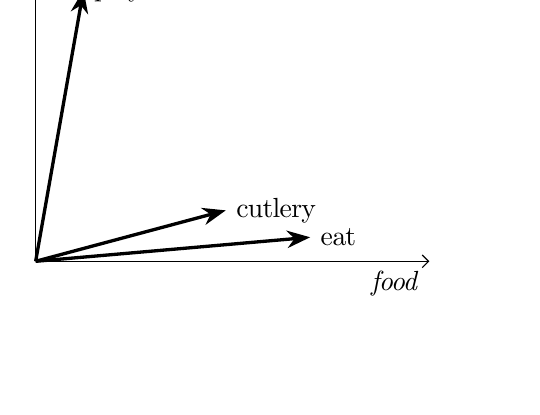
\begin{tikzpicture}[
            > = Straight Barb,
phasor/.style = {very thick,-{Stealth}},
angles/.style = {draw, <->, angle eccentricity=1,
                 right, angle radius=7mm}
                        ]
% coordinates
    \draw[->] (0,0) -- (5,0) coordinate (x) node[below left] {$\mathit{food}$};
    \draw[->] (0,0) -- (0,4) node[below left] (y) {$\mathit{tennis}$};
% phasors
    \draw[phasor] (0,0) -- (80:3.5) coordinate (i)  node[right] {play};% used polar coordinates
    \draw[phasor] (0,0) -- (15:2.5) coordinate (v)  node[right] {cutlery};% used polar coordinates
    \draw[phasor] (0,0) -- (5:3.5) coordinate (i)  node[right] {eat};% used polar coordinates
% angles drawn by pic
\coordinate (X)   at (0,0);
\end{tikzpicture}
\caption{A depiction of words in a 2-D semantic space}
\end{center}
\label{fig:dseg}
\end{figure}
\subsubsection{Measuring Compositionality}
Given that the meaning of a word is predictable from its context, we can use it to predict an MWE's compositionality \citep{Bannard2003,Mccarthy2003,Reddy2011}. If we see that an MWE is used in similar contexts as its components, we can deduce that it is compositional. To do that, we calculate the similarity between the semantic vector of the MWE and that of its constituents.

Distributional similarity is a good general-purpose approach to this problem because it can be applied to any language, as long as there is a large enough corpus to identify all the tokens being considered. 

\cite{Lin1999} proposed that we could analyse the compositionality of an MWE by substituting its constituents for lexically similar variants. \cite{Bannard2003} used Latent Semantic Analysis (LSA) to analyse the relationships between a kind of MWE called Verb Particle Constructions \citep{Wasow2003} and their constituents and found that it was superior to the previously used lexical substitutability approach. LSA follows the \textit{distributional hypothesis} discussed above to generate a set of concepts that relate the MWE to its component words by assuming that words with similar meanings will occur in similar text spans. In contrast to \cite{Bannard2003}, \cite{Mccarthy2003} employed distributional similarity to find a specified number of the most semantically similar terms to the VPC and its constituents. They then measured the overlap between the semantically similar terms to the VPC and its components. \cite{Reddy2011} used distributional similarity to measure how literal the constituents within the NCs were by performing a weighted sum of the representations of each of the constituents and calculating the similarity between the resultant vector and that of the NC.

While distributional similarity is a promising approach, given how well it performs despite being unsupervised, it is not without its shortcomings:
\begin{enumerate}
    \item As seen in \secref{sec:intro}, the compositionality of some MWEs may be ambiguous without context (for example \textit{silver screen, piece of cake, red carpet}). Distributional similarity, in such a case, would generate either noisy vectors that represent both uses of the collocation or highly biased vectors that always lean towards its more popular sense.
    \item Language is complicated and we often observe polysemy (the existence of many possible meanings for a word or phrase, for example the word \textit{bridge} which could mean a span, the card game or the upper deck of a ship) and homonymy (words with different meanings that are identical in spelling or pronunciation, for example \textit{pen} that could mean either \textit{a writing instrument} or \textit{a holding area for animals}). Distributional similarity is not equipped to handle and/or determine which sense of the component is intended, especially in the case of polysemy.
\end{enumerate}

\subsection{Word Embeddings}
Word embeddings are a particular instantiation of distributional semantics via representation learning, whereby contextual similarity is used to map words into a continuous n-dimensional space. There are many different methods to generate these representations-- neural networks \citep{Bengio2003}, principle component analysis \citep{Lebret2013}, matrix factorization \citep{Jeffrey2014} and log-linear models \citep{Mikolov2013}.

While \cite{Coll2008} were the first to propose the utilization of word embeddings in an application, they are now widely used across a range of NLP tasks, such as identifying various syntactic and semantic relations \citep{Mikolov2013}, dependency parsing \citep{Bansal2014}, named-entity recognition \citep{Passos2014} and translation \citep{Zou2013}.

\cite{Salehi2015} were the first to investigate the use of word embeddings to predict the compositionality of MWEs and achieved state-of-the-art results over the English NC dataset from \cite{Reddy2011}. Since their work utilized word-level embeddings (see \secref{sec:emb}), they needed to perform a token-level identification of the MWEs in the training corpus. This method was recently tuned variously by \cite{Cordeiro2019} and remains state-of-the-art for the task of MWE compositionality prediction, but the caveat still remains. This is not ideal, as it means the model will need to be retrained for a new set of MWEs (as the tokenisation will necessarily change). It also requires ``complete'' knowledge of the MWEs before the training step, which is impractical in most cases. \cite{Hakimi2018} tried to circumvent this by using character-level embeddings (see \secref{sec:emb}) and achieved significant correlations between their similarity scores and the human annotations of the data from \cite{Reddy2011}.

\noindent
The next section provides a detailed discussion of word embeddings.

\section{Language Embedding Models}
\label{sec:emb}
Language models compute the probability distribution of the next word in a sequence given the sequence of previous words. With the help of these techniques, we are able to extract information regarding the syntactic and semantic relationships between words better than has been possible previously using traditional word representations (like one-hot encoding and bag-of-words).

Embedding techniques represent a text (word, sentence or document) as multidimensional continuous floating point numbers that each capture a dimension of the text's meaning, where semantically similar texts are mapped to proximate points in geometric space. Each dimension of the vector represents a meaning, i.e. the text's numerical weight on that dimension captures the closeness of its association to that meaning. Thus, the semantics of a text are embedded across the dimensions of its vector, which make semantic associations (like the aforementioned) possible.
\subsection{Word-level}
Word-level embeddings, as the name suggests, embed words in vector space. These embeddings are generated using one of two methods:
\begin{itemize}
\item \textbf{Continuous bag-of-words (CBOW):} This method predicts a target word using its context. It is relatively quick to train.
\item \textbf{SkipGram:} This method uses a word to predict a target context. It produces more accurate results on larger datasets and infrequent words, though it takes longer to train.
\end{itemize}
\begin{figure}[h!]
\begin{center}
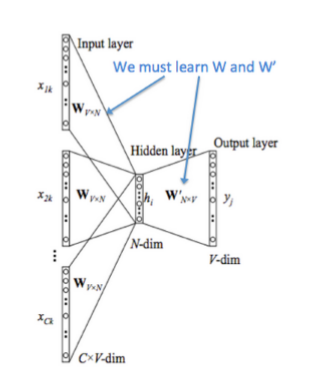
\includegraphics[width=0.4\textwidth]{Figures/CBOW.PNG}
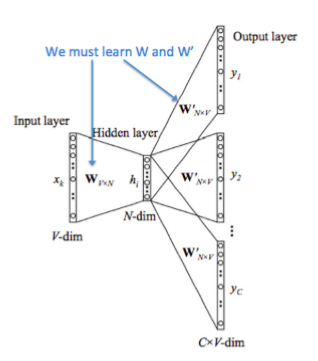
\includegraphics[width=0.4\textwidth]{Figures/SkipGram.PNG}
\caption{CBOW vs. SkipGram methods of training \footnotemark}
\end{center}
\end{figure}
\footnotetext{\url{http://cs224d.stanford.edu/lecture_notes/LectureNotes1.pdf}}

\paragraph{\wordtovec} \wordtovec \citep{Mikolov2013b} is a two-layer neural net that processes text. Its input is a text corpus and its output is a set of feature vectors for word types in that corpus. It treats words as distinct states and looks for the transitional probabilities between those states, i.e. the likelihood that they will co-occur. \wordtovec groups the vectors of similar words in vector space and can, thus, detect similarities mathematically. It does this by using the numerical representations of features such as the context of individual words to generate the word vectors. The model adjusts the vector components if it is unable to make accurate predictions of the word's context based on its assigned feature vector in the case of SkipGram (vice versa for CBOW). That is how the vectors of words judged to be similar based on their context are plotted closer together.

\wordtovec is widely used among the NLP research community to calculate the similarity of words. This can be applied to information retrieval tasks, for example, where it can be used to calculate the similarity between query vectors and their candidate documents \citep{Roy2018}.

\subsection{Character-level}
In a character-level embedding model, the vector for a word is constructed from the character n-grams that compose it. Since these are shared across words, these models can even generate embeddings for word they haven't encountered before. They also tend to handle infrequent words better, where word embedding models suffer from lack of sufficient training.

\paragraph{\fasttext}
\fasttext \citep{Bojanowski2017} is an adaptation of the \wordtovec model that seeks to enrich its word vectors with subword information. It composes a word vector by summing the n-gram vectors constituting the word. \fasttext supports training CBOW or Skip-gram models using negative sampling, softmax or hierarchical softmax loss functions. It also stores the positional information of these n-grams embedded in the resultant vector. For example, for the word \textit{clean}, with n = 2, the \fasttext representations for the character n-grams is \textit{$\langle$c,cl,le,ea,an,n$\rangle$}, where $\langle$ and $\rangle$ are boundary symbols to help distinguish between n-grams of a word and entire words. For example, the word \textit{an} would be represented as \textit{$\langle$an$\rangle$} to distinguish it from the identical n-gram \textit{an} observed in \textit{clean} and other such words. Inherently, this also allows you to capture meaning for suffixes/prefixes.
Therefore, the vector for the the word \textit{today} will not be the same as the vector for its misspelled variant \textit{tdoay} as the n-grams constituting both these vectors are very different.

\fasttext is widely used in text classification tasks like spam detection and sentiment analysis.

\subsection{Document-level}
Document-level embeddings are unsupervised methods for learning distributed representations of spans of text (sentences, paragraphs or documents). They are useful for generalisations as they concern themselves primarily with representing the semantics of the text \citep{Le2014}.
\paragraph{\doctovec}
Paragraph Vector (\doctovec) is an extension of \wordtovec that aims to learn how to project a document into a latent d-dimensional space regardless of its length. It works by taking context words and a paragraph ID as input and predicts a word central to a randomly sampled set of consecutive words from the paragraph \citep{Lau:Baldwin:2016b}. This is essentially the \wordtovec CBOW model that uses one extra vector to represent the paragraph ID, which is unique for each document (\figref{fig:d2vVSw2v}). Similarly, the \doctovec SkipGram model uses the paragraph vector to predict context words, or words that it expects to be observed in the document.
\begin{figure}[h!]
\begin{center}
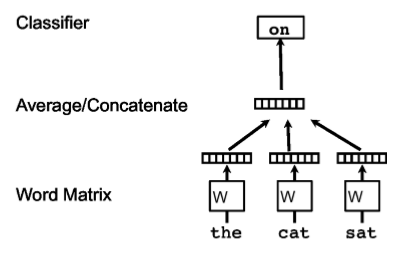
\includegraphics[width=0.4\textwidth]{Figures/w2vCBOW.PNG}
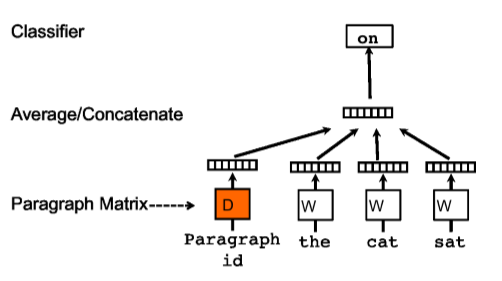
\includegraphics[width=0.4\textwidth]{Figures/d2vCBOW.PNG}
\caption{\wordtovec CBOW vs \doctovec CBOW models \citep{Le2014}}
\label{fig:d2vVSw2v}
\end{center}
\end{figure}
This paragraph vector is trained along with the word vector to hold a numerical representation of the document it identifies. This model, called \textit{Distributed Memory version of Paragraph Vector (PV-DM)} is actually faster (as opposed to \wordtovec word averaging) and consumes less memory, since it does not retain the individual word vectors.

\doctovec has been shown to work well in multi-class text classification and sentiment analysis problems.

\paragraph{\infersent}
\infersent \citep{Conneau2017} is a sentence embedding method trained on natural language inference data to provide semantic representations of English text. It uses the Stanford Natural Language Inference (SNLI) Corpus, a set of 570,000 pairs of sentences labelled one of 3 categories: neutral, contradiction and entailment, to train a classifier over a sentence encoder \figref{fig:inferSent}. Both the sentences of a pair are encoded using the same encoder, while the classifier is trained on the pair representation constructed from the two individual sentence embeddings. \cite{Conneau2017} adopt a bi-directional LSTM that encodes the sentences using a max-pooling operator.
\begin{figure}[h!]
\begin{center}
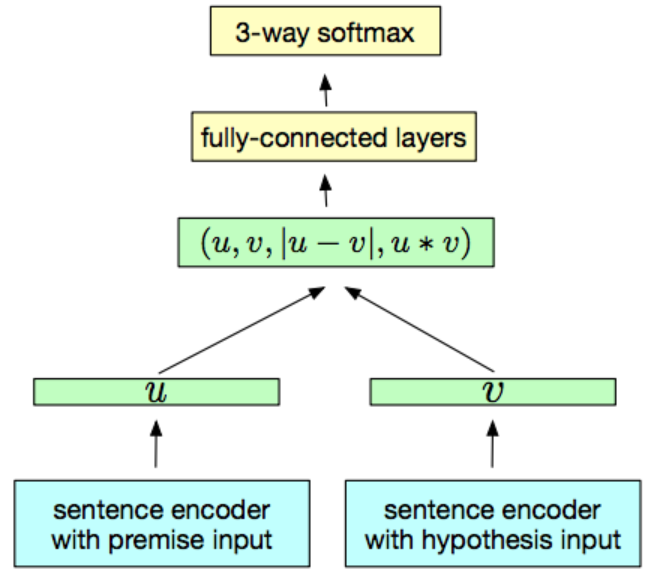
\includegraphics[width=0.5\textwidth]{Figures/InferSent.PNG}
\caption{The sentence encoder and classifier of \infersent \citep{Conneau2017}}
\label{fig:inferSent}
\end{center}
\end{figure}
\infersent has been shown to work well on transfer learning tasks-- a model that is trained to solve one task used to solve another \citep{Conneau2017}.

\subsection{Contextualised Embeddings}
The models so far exhibit one fundamental flaw-- they generate the same embedding for a word regardless of  its context. Consider again the word \textit{bridge} that displays polysemy and would be represented with the same vector embedding despite its difference in meaning in the following sentences:
\begin{enumerate}
\item \textit{The \underline{bridge} is under construction.}
\item \textit{I met John for a game of \underline{bridge}.}
\item \textit{We need to \underline{bridge} the gap between the rich and poor.}
\end{enumerate}

\noindent
Contextualised word embeddings aim to capture word semantics in different contexts to address the context-dependent nature of such words.

\paragraph{\elmo}
\elmo (Embeddings from Language Models) is an LSTM-based model that is trained on a corpus to generate a vector representation of a word using the hidden states of the LSTM \citep{Peters2018}. The language model is trained by reading the sentences both forward and backward, i.e. it learns to predict the next word given the past words, as well as the previous word given the future words-- effectively performing the task of two models. However, rather than using the embedding of the words from a word embedding matrix, each token is converted to an appropriate representation using character embeddings, which is then run through a convolutional layer using a number of filters, followed by a max-pool layer.The resultant representation is passed through a 2-layer highway network before being provided as the input to the LSTM layer.
There are a number of reasons for these transformations:
\begin{enumerate}
    \item Character embeddings are preferred because they are capable of picking up morphological features that word-level embeddings could miss.
    \item The convolution filters detect n-gram features that build more powerful representations.
    \item The highway network layers allow the information to be transferred more smoothly. 
\end{enumerate}

By using a multi-layer LSTM, which also considers the output sequence of the previous layer as input (in addition to the plain sequence of words), each layer of the model is able to learn a different characteristic of the language.

\elmo has been shown to work impressively well on tasks ranging from question-answering to sentiment analysis \citep{Peters2018}.

\paragraph{\bert}
Consider the sentence \textit{I need to make a bank deposit}. A left unidirectional contextual model would use the context words on the left of \textit{bank} (\textit{I, need, to, make, a}) to contextualise it and would leave out \textit{deposit}. A right unidirectional model would only use \textit{deposit} and leave out the rest. In either case, we may not be able to capture the word's context accurately. \elmo attempts to handle this by stacking a forward and backward LSTM.

As the name suggests, \bert (Bidirectional Encoder Representations from Transformers) uses birectional transformers to solve the same problem. A transformer is an encoder-decoder architecture model that uses attention mechanisms to project the whole sequence of text to the decoder at once rather than sequentially. They are preferred over conventional sequential models like LSTMs and RNNs because they model long term dependencies among tokens more effectively and eliminate the need for the sequential dependency on previous tokens. \bert models text by employing a technique known as \textit{masked language modelling} to mask 15\% of the words in a sentence and then forces itself to learn how to use their positional information to infer them. It does this because it utilises only the encoders from transformers, which would otherwise ``see'' all the words during the encoding phase.

\bert has been shown to work as well as \elmo on a range of tasks, including non-linguistic tasks like quantitative trading.

\paragraph{\flair}
\flair \citep{Akbik2018} is a sequence labeling architecture built on top of neural language modeling and trained without any explicit notion of words. Therefore, it models a word as a string of characters solely dependent on its contextual use, without regard for its meaning. It feeds a sentence as input into a pre-trained bidirectional character language model to retrieve a contextual embedding for each word in the sentence. The embedding is created by extracting the cell states for the first and last characters of the word. This word embedding is then passed into a bidrectional LSTM-CRF sequence labeller.

\begin{figure}[h!]
\begin{center}
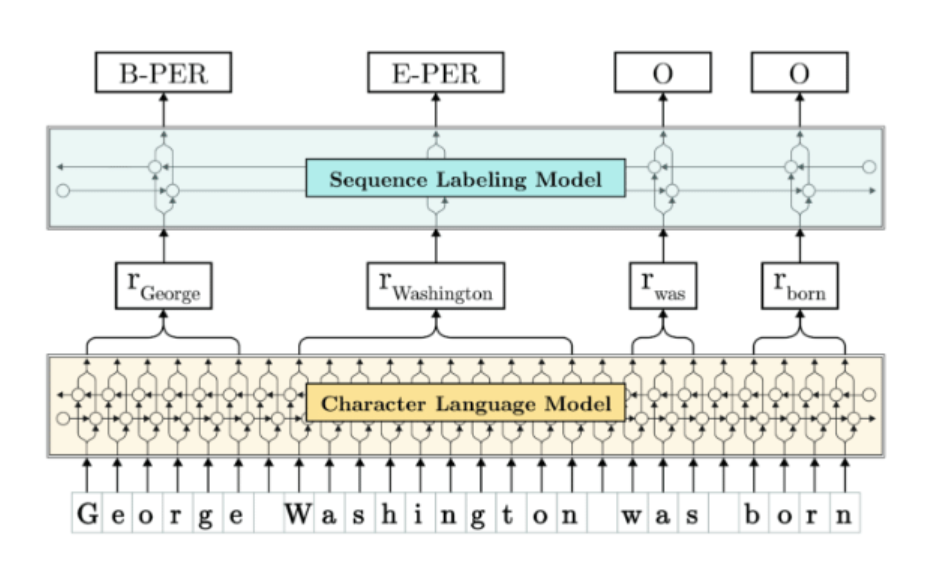
\includegraphics[width=0.8\textwidth]{Figures/Flair.PNG}
\caption{\flair performing NER tagging\footnotemark}
\label{fig:flair}
\end{center}
\end{figure}
\footnotetext{\url{https://research.zalando.com/welcome/mission/research-projects/flair-nlp/}}
\flair has been shown to outperfrom previous state-of-the-art embedding models in various downstream tasks like sequence labelling and named-entity recognition, as seen in \figref{fig:flair} \citep{Akbik2018}.

\section{Summary}
In this chapter, we provided a brief overview on multiword expressions and their importance. We discussed the prediction of the compositionality of such expressions and detailed some of the existing methods used in this task. Finally, we described some of the modern language embedding models and their use in natural language processing.

In the next chapter, we will employ the embedding models discussed to model the compositionality of MWEs and compare their performance.

%\section{Multi-task Learning}
%\label{sec:MTL}
%\cite{Kazuma2016},\cite{Coll2018}, \cite{Subramanian2018}, \cite{McCann2018}, \cite{Sanh2018}, \cite{Fares2018}, 

\chapter{Comparative Study of Language Embedding Models}
\section{Introduction}
In this chapter, we evaluate the performance of the various embedding models discussed in \secref{sec:emb} in predicting the compositionality of MWEs; specifically English binary noun compounds (NN) and adjective-noun pairs (ADJ-N). Our results show that \wordtovec performs the best, followed by \fasttext and \infersent. We discover, surprisingly, that recently-proposed contextualised embedding models such as \bert and \elmo do not perform impressively in this task. We also experiment with using paraphrases to aid prediction and obtain promising results.

\section{Datasets}
\label{sec:datasets}
We use four datasets for our experiments and evaluate each model's performance using Pearson's correlation coefficient ($r$) to compare the similarity scores obtained with the annotated compositionality scores provided.

\paragraph{\reddy}
The dataset of \cite{Reddy2011} contains 90 English binary noun compounds, along with human-annotated scores of their overall compositionality and component-specific compositionality, ranging from 0 (completely non-compositional) to 5 (completely compositional). 30 annotators worked over Amazon Mechanical Turk to select the definition of the compound noun that occured most frequently in the 5 example sentences provided and score the compound for literality based on the most frequent definition. The final compositionality scores were the average of the annotations with Spearman's $\rho$ greater than 0.6, as well as other annotions that were within the range of $\pm$1.5 from the task's mean.

\noindent
For our experiments, we consider the overall compositionality scores only.

\paragraph{\ramisch}
Similar to \reddy, the English dataset of \cite{Ramisch2016} contains 90 binary noun compounds with annotated scores of compositionality ranging from 0 to 5, both overall and component-specific. It also contains a list of paraphrases for each NC, presented in decreasing order of popularity among the annotators. The scores were derived from 15 human intelligence tasks, wherein annotators were made to perform 5 subtasks for each compound noun:
\begin{enumerate}
    \item Read the noun compound itself
    \item Read 3 sentences containing the compound noun
    \item Provide 2-3 paraphrases for the noun compound based on its meaning as seen in the sentences
    \item Provide a judgement score from 0-5 using a Likert scale of how much of the meaning of the compound comes from the modifier and head separately
    \item Provide a judgement score from 0-5 using a Likert scale of how much the meaning of the compound comes from its components overall
\end{enumerate}
The final scores provided are an average of the annotations.

\noindent
We use only the overall compositionality scores and the paraphrase data in our work.
\paragraph{\discoj}
The English dataset from the DiSCo shared task \citep{Disco2011} contains a total of 348 binary compounds, comprising adjective--noun, verb--noun\textsubscript{subj} and verb--noun\textsubscript{obj} pairs, along with their overall compositionality rating ranging from 0 to 100. The phrases were extracted semi-automatically and their relations were assigned by patterns and checked manually. The compositionality scores were collected from Amazon Mechanical Turk, where workers were presented with 4-5 randomly sampled sentences from the UK English WACKy corpora. The standard number of judgments per target phrase was 20. The final scores were computed by averaging over all the judgements per phrase.

\noindent
We focus on the 145 adjective--noun pairs in this study.
\paragraph{\farahm}
This dataset comprises 1042 English binary noun compounds with four accompanying compositionality labels of either 0 or 1. The four human experts were asked to label the pair 0 for compositional and 1 for non-compositional. Unlike the previous datasets, \farahm presents a binary classification task \citep{Farah2015c}. In addition to compositionality labels, each noun compound also has four conventionalization labels of either 0 (unconventional) or 1 (conventional). 

\noindent
For our experiments, we compute the average of the four labels to produce a score ranging from [0,1] to match our regression task. \figref{fig:datasets} shows a section of the datasets used in this study.
\begin{figure*}[h!]
\centering
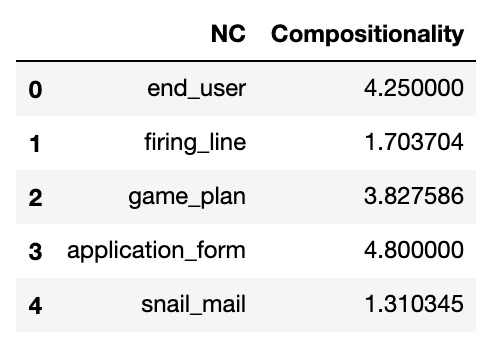
\includegraphics[width = .32\textwidth,]{Figures/reddy.PNG}
\small (a) \reddy
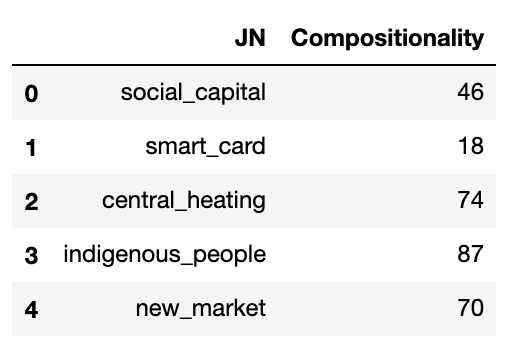
\includegraphics[width = .33\textwidth]{Figures/disco_j.PNG}
\small (b) \discoj
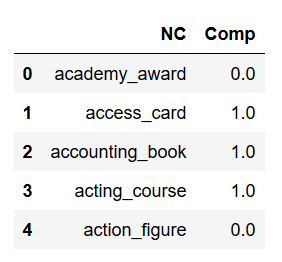
\includegraphics[width = .25\textwidth]{Figures/farahm_after.PNG}
\small (c) \farahm
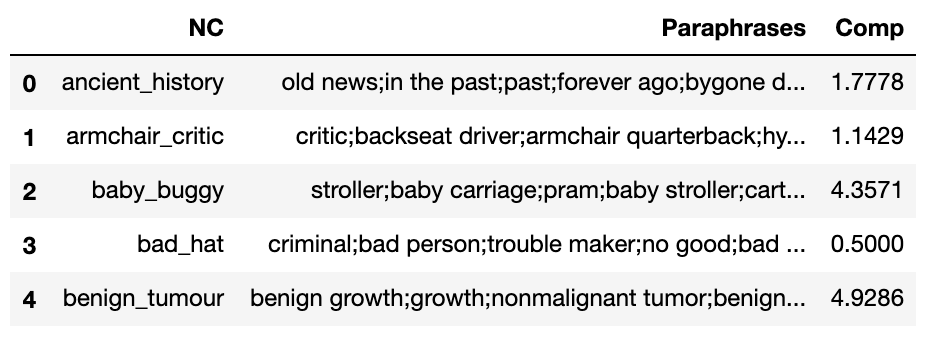
\includegraphics[width = .7\textwidth]{Figures/ramisch.PNG}
\small (d) \ramisch
\caption{Datasets used in this study}
\label{fig:datasets}
\end{figure*}

\begin{table}[t]
\begin{center}
\begin{tabular}{lSS@{\,}l}
  \toprule
  Dataset & $\mu$ & $\sigma$ \\
  \midrule
  \reddy & 53.2 & 30.0 \\
  \ramisch & 52.6 & 35.0 \\
  \discoj & 68.1 & 21.7 \\
  \farahm &  83.1 & 31.8 \\
  \midrule
  Overall & 64.25 & 29.6 \\
\bottomrule
\end{tabular}
\caption{Mean ($\mu$) and standard deviation ($\sigma$) of the compositionality scores of the datasets, over a normalised range $[0,100]$.}
\label{tab:stats}
\end{center}
\end{table}

\bigskip
\noindent
The summary of compositionality scores across the three datasets in \tabref{tab:stats} indicates there is a reasonable distribution of data in terms of compositionality, with \reddy and \ramisch being roughly comparable and covering a broad (and somewhat balanced) spectrum of compositionalities, while \discoj is more skewed towards compositional usages, with lower standard deviation. \farahm's mean shows us it has a higher distribution of compositional noun compounds.

Although we conduct our experiments on English datasets, they can be applied to other languages as we do not perform any kind of language-specific manipulation of the data.

\section{Methodology}
\label{sec:method}
We compute the overall compositionality of an MWE using three broad metrics-- direct composition, paraphrase similarity, and a combined metric. In all experiments, the similarity of a pair of vectors is measured using cosine similarity.

\subsection{Direct Combination}
\label{sec:direct}
Intuitively, an MWE appearing in similar contexts to its component words is likely to be compositional. Following \cite{Salehi2015} and \cite{Reddy2011}, we compare the vector representation of an MWE with that of its component words directly in one of two ways:
\begin{enumerate}
    \item We perform an element-wise sum to obtain a `combined' vector, which is then compared with the vector of the MWE
    \begin{eqnarray}
    \presum =  \cos(\MWEvec, \MWEonevec + \MWEtwovec)
\end{eqnarray}
    \item We combine the scores obtained by individually comparing the vector of the MWE with that of its components post-hoc, via a weighted sum
    \begin{eqnarray}
    \postsum = & \alpha \cos(\MWEvec, \MWEonevec) +  
     (1 - \alpha) \cos(\MWEvec, \MWEtwovec)
    \end{eqnarray}
\end{enumerate}

Here, \MWEvec, \MWEonevec, and \MWEtwovec are the embeddings for the combined MWE, first component and second component, respectively. $\MWEonevec + \MWEtwovec$ is the element-wise sum of the vectors of each of the component words of the MWE; and $\alpha \in [0,1]$ is a scalar which allows us to vary the weight of the respective components in predicting the compositionality of the compound. This helps us effectively capture the compositionality of the MWE with regards to each of its individual constituents. We do not perform any tuning of $\alpha$ over held-out data and are, as such, overfitting as we select the best-performing $\alpha$ post hoc. We do, however, present analysis of hyper-parameter sensitivity in \secref{sec:results}.

It is noteworthy that while all methods are presented and evaluated in terms of two-element MWEs in this work, they are trivially generalisable to multi-element MWEs.

\subsection{Paraphrase Similarity}
Another intuition is that a compositional MWE would appear in similar contexts to the component words of its paraphrases, since each paraphrase provides an interpretation of its semantics (for e.g. the paraphrases \textit{``old times''} and \textit{``long long ago''} offer a rough explanation of the meaning of the MWE \textit{``ancient history''}). The \ramisch dataset (described in \secref{sec:datasets}) provides one or more paraphrases for each MWE. We calculate the similarity of the embeddings of the MWE and its paraphrases using three formulae:
\begin{eqnarray}
\firstpara = & \cos(\MWEvec, \paravec[1])\\
\avgparapre = & \cos(\MWEvec, \sum_i \paravec[i])\\
\avgparapost = & \frac{1}{N} \sum_{i=1}^N \cos(\MWEvec, \paravec[i])
\end{eqnarray}
where \paravec[1] and \paravec[i] denote the embeddings of the first (most popular) and $i$-th paraphrases, respectively.

In the case of \avgparapost, we considered computing the maximum instead of the average (as we report here) of the similarity scores between each paraphrase and its MWE, following the intuition that an MWE would be similar to at least one reported paraphrase, rather than all of them. However, the results for the average similarity were empirically higher across models.
\subsection{Combined Metric}
Finally, we combine the results obtained from the aforementioned methods:
\begin{eqnarray}
  \begin{split}
    \combined = & \beta\max(\presum, \postsum) + \\
    & (1 - \beta)\max(\firstpara, \avgparapre, \avgparapost) \\
  \end{split}
\end{eqnarray}
$\beta\in[0,1]$ is a scalar weighting factor used to balance the effects of the two methods, in order to measure the extent to which the compositionality is determined by each of the methods. We use the $\max$ operator here to combine the sub-methods for each of the direct composition and paraphrase methods since all methods tend to underestimate the compositionality. It was also empirically found to be superior to taking the mean.

\section{Experiments}
We implement the metrics detailed above using each of the language embedding models discussed in \secref{sec:emb} and compare their performance. Where available, we made use of pretrained models as is standard practice in NLP. As the different models are trained on different corpora, we are not attempting to perform a controlled comparative evaluation of the different models, so much as a comparison of the standard pretrained versions of each. If we were to retrain our own models over a standard dataset, such as English Wikipedia\textsuperscript{\ref{wiki}}, we would expect the results for the document-level embedding models in particular to drop.

\paragraph{\wordtovec} \wordtovec is a word-level embedding model. Therefore, if fed with one of our MWEs, it will perform delimiting by space and generate embeddings for each of its component words instead. To circumvent this, we would like to treat the MWE as a single word (spaces removed) and generate a single representative vector embedding. For instance, we would generate an embedding for \textit{``closeshave''} to represent the MWE \textit{``close shave''}. However, another issue with \wordtovec is that it is incapable of handling out-of-vocabulary words (OOVs) and, hence, would fail to generate a representation for \textit{``closeshave''} if it has never seen it before (which is understandable, given all occurrences of the MWE in the training corpus would include the space). The solution then is to remove the space from all occurrences of the MWEs in the training corpus.

We trained the gensim implementation of \wordtovec on a recent English Wikipedia dump,\footnote{\label{wiki}Dated 07-Jan-2019} after pre-processing it (removing the formatting and punctuation) and, following \cite{Salehi2015}, concatenating each occurence of the MWE in our datasets (i.e., every occurence of \textit{``close shave''} in the corpus becomes \textit{``closeshave''}), making an over-optimistic assumption that every occurring collocation of the component words represent the MWE in question. The resultant \wordtovec model generates vector representations with 300 dimensions using SkipGram and a minimum count and window size of 5.

In cases where the model fails to generate an embedding for the expression due to low token frequency, and we observe 2, 8 and 25 cases of this in \reddy, \ramisch and \discoj, respectively, we assign a default compositionality score of 0.5 (neutral; based on a range of [0,1]). For paraphrases, we compute an element-wise sum of the embeddings for each of the component words to serve as the embedding of the phrase. We do this because token-level identification of each paraphrase in the training corpus is not feasible and the element-wise sum approach is consistent with the MWE compositionality prediction approaches of \cite{Salehi2015} and \cite{Reddy2011} and a paraphrase could be thought of as an MWE in its own right.

\paragraph{\fasttext}
Since \fasttext represents each word as a bag of its ngrams, it is capable of generating embeddings for OOV terms as well. Therefore, no manipulation of the training corpus is necessary. However, like \wordtovec, it performs whitespace delimiting and we therefore need to preprocess our MWEs and paraphrases the same way as stated above to derive a \textit{fused compound} (i.e. we use the embedding for \textit{``closeshave''} to represent \textit{``close shave''}).

We used the 300-dimensional \fasttext model pre-trained on Common Crawl and Wikipedia using CBOW (\fasttextpre), as well as one trained over our Wikipedia corpus\textsuperscript{\ref{wiki}} using skip-gram (\fasttext).

\paragraph{\doctovec}
Since \doctovec is a document-level embedding, we treat the MWE as a two-word document, as well as each of its components as single word documents to generate their embeddings.

We used the gensim implementation of \doctovec pretrained on Wikipedia data using the \wordtovec skip-gram models pretrained on Wikipedia and AP News.\footnote{\url{https://github.com/jhlau/doc2vec}}

\paragraph{\infersent}
Similar to the approach used in \doctovec, we treat the MWE as a two-word sentence and its components as single word sentences to generate their embeddings using \infersent, which is a sentence-level embedding.

We used two pretrained versions of \infersent: \infersent[\glove] and \infersent[\fasttext]. Each generates a representation of 4096 dimensions, trained over the 1,000,000 most popular English words using \glove \citep{Jeffrey2014} and \fasttext, respectively.

\paragraph{Contextualised Embeddings}
We used the pretrained implementations of \elmo, \bert and \flair available in the \flair framework.\footnote{\url{https://github.com/zalandoresearch/flair}}

We used sentences extracted from the Brown corpus where available in order to derive contextualised interpretations. We used literary context as it was more likely to have instances of the more idiomatic or non-compositional MWEs, as opposed to news or Wikipedia corpora. We extracted 25 sentences at random for each MWE, except where there were fewer sentences in the corpus.

We also included a naive context-independent implementation of \elmo, \bert and \flair in our study, consistent with the other models. This also helped us test our intuition that the relative compositionality of even novel compounds could potentially be predicted from its component words alone. Consider for instance the unseen expression \textit{``giraffe potato''}, which could have the plausible compositional interpretation of a potato shaped like a giraffe (considering contexts like \textit{round potato}, say), while \textit{``couch intelligence''} might have no natural interpretation given its context and could, therefore, be assumed to have a non-compositional meaning.

%Nav: clean up diagrams and tables, rewrite the section to include insights on farahm dataset also
\section{Results and Discussion}
\label{sec:results}
The results from our experiments on the \reddy,  \discoj, \farahm and \ramisch datasets can be found in \tabref[s]{tab:reddy},\ref{tab:discoj}, \ref{tab:farahm} and \ref{tab:ramisch}, respectively, with the best performing $\alpha$s and $\beta$s mentioned for each embedding model.

\begin{table}[t]
\minipage{0.45\textwidth}
\begin{tabular}{lSS@{\,}l}
  \toprule
  Emb.\ method        & {\presum}  & \multicolumn{2}{c}{\postsum} \\
  \midrule
  \wordtovec & \B 0.634 & \B 0.622 & ($\alpha$ = 0.6) \\
  \fasttextpre & 0.223 & 0.285 & ($\alpha$ = 0.3) \\
  \fasttext & 0.217 & 0.287 & ($\alpha$ = 0.3) \\
  \doctovec & -0.049 & 0.025 & ($\alpha$ = 0.0) \\
  \infersent[\glove] & 0.413 & 0.500 & ($\alpha$ = 0.5) \\
  \infersent[\fasttext] & 0.401 & 0.527 & ($\alpha$ = 0.6) \\
  \elmo & 0.339 & 0.406 & ($\alpha$ = 0.5) \\
  \elmocon & 0.363 & 0.406 & ($\alpha$ = 0.5) \\
  \bert & 0.304 & 0.352 & ($\alpha$ = 0.2) \\
  \bertcon & 0.311 & 0.372 & ($\alpha$ = 0.2) \\
  \flair & -0.127 & 0.024 & ($\alpha$ = 0.0) \\
  \flaircon & 0.002 & 0.102 & ($\alpha$ = 0.0) \\
\bottomrule
\end{tabular}
\caption{Pearson correlation coefficient for compositionality prediction results on the \reddy dataset.}
\label{tab:reddy}
\endminipage\hfill
\minipage{0.45\textwidth}
\begin{tabular}{lSS@{\,}l}
  \toprule
  Emb.\ method        & {\presum}  & \multicolumn{2}{c}{\postsum} \\
  \midrule
  \wordtovec & \B 0.427 & \B 0.419 & ($\alpha$ = 0.4) \\
  \fasttextpre & 0.339 & 0.353 & ($\alpha$ = 0.6) \\
  \fasttext & 0.374 & 0.419 & ($\alpha$ = 0.4) \\
  \doctovec & -0.023 & 0.003 & ($\alpha$ = 0.0) \\
  \infersent[\glove] & 0.321 & 0.315 & ($\alpha$ = 0.4) \\
  \infersent[\fasttext] & 0.001 & 0.202 & ($\alpha$ = 1.0) \\
  \elmo & 0.253 & 0.287 & ($\alpha$ = 0.5) \\
  \elmocon & 0.282 & 0.316 & ($\alpha$ = 0.5) \\
  \bert & 0.154 & 0.177 & ($\alpha$ = 0.3) \\
  \bertcon & 0.166 & 0.181 & ($\alpha$ = 0.3) \\
  \flair & 0.261 & 0.291 & ($\alpha$ = 0.4) \\
  \flaircon & 0.272 & 0.303 & ($\alpha$ = 0.4)  \\
\bottomrule
\end{tabular}
\caption{Pearson correlation coefficient for compositionality prediction results on the \discoj[ADJ] dataset.}
\label{tab:discoj}
\endminipage\hfill
\end{table}

\begin{table}[t]
\begin{center}
\begin{tabular}{lSS@{\,}l}
  \toprule
  Emb.\ method        & {\presum}  & \multicolumn{2}{c}{\postsum} \\
  \midrule
  \wordtovec & .244 & \B .35 & ($\alpha$ = 0.9) \\
  \fasttextpre & .197 & .291 & ($\alpha$ = 0.8) \\
  \fasttext & .203 & .295 & ($\alpha$ = 0.8) \\
  \doctovec & .083 & .088 & ($\alpha$ = 0.8) \\
  \infersent[\glove] & .002 & .010 & ($\alpha$ = 1.0) \\
  \infersent[\fasttext] & -.059 & .019 & ($\alpha$ = 1.0) \\
  \elmo & \B.283 & .278 & ($\alpha$ = 0.5) \\
  \elmocon & .291 & .280 & ($\alpha$ = 0.5) \\
  \bert & .176 & .193 & ($\alpha$ = 0.9) \\
  \bertcon & .179 & .191 & ($\alpha$ = 0.9) \\
  \flair & .222 & .23 & ($\alpha$ = 0.6) \\
  \flaircon & .229 & .247 & ($\alpha$ = 0.6) \\
\bottomrule
\end{tabular}
\caption{Pearson correlation coefficient for compositionality prediction results on the \farahm dataset.}
\label{tab:farahm}
\end{center}
\end{table}

\begin{table*}[t!]
\begin{center}
\begin{tabular}{lSS@{\,}lSSSS@{\,}l}
\toprule
  Emb.\ method        & {\presum}  & \multicolumn{2}{c}{\postsum} & {\firstpara} & {\avgparapre} & {\avgparapost} & \multicolumn{2}{c}{\combined} \\
  \midrule
  \wordtovec & \B 0.581 & \B 0.571 & ($\alpha$ = 0.6) & 0.443 & 0.510 & 0.504 & 0.677 & ($\beta$ = 0.9) \\
  \fasttextpre & 0.395 & 0.446 & ($\alpha$ = 0.7) & 0.242 & 0.531 & 0.703 & 0.703 & ($\beta$ = 0.0) \\
  \fasttext & 0.464 & 0.532 & ($\alpha$ = 0.7) & 0.548 & 0.613 & 0.673 & 0.673 & ($\beta$ = 0.0) \\
   \doctovec & -0.157 & 0.039 & ($\alpha$ = 1.0) & 0.388 & 0.334 & 0.373 & 0.419 & ($\beta$ = 0.3) \\
   \infersent[\glove] & 0.321 & 0.427 & ($\alpha$ = 0.7) & \B 0.636 & 0.700 & \B 0.741 & \B 0.783 & ($\beta$ = 0.5) \\
  \infersent[\fasttext] & 0.169 & 0.221 & ($\alpha$ = 0.6) & 0.488 & \B 0.712 & 0.636 & 0.712 & ($\beta$ = 0.0) \\
  \elmo & 0.420 & 0.459 & ($\alpha$ = 0.6) & 0.361 & 0.488 & 0.546 & 0.546 & ($\beta$ = 0.2) \\
  \elmocon & 0.448 & 0.486 & ($\alpha$ = 0.6) & 0.366 & 0.486 & 0.550 & 0.621 & ($\beta$ = 0.2) \\
  \bert & 0.071 & 0.086 & ($\alpha$ = 1.0) & 0.242 & 0.531 & 0.583 & 0.583 & ($\beta$ = 0.0) \\
  \bertcon & 0.087 & 0.107 & ($\alpha$ = 1.0) & 0.257 & 0.541 & 0.598 & 0.598 & ($\beta$ = 0.0) \\
  \flair & 0.165 & 0.295 & ($\alpha$ = 0.1) & 0.334 & 0.399 & 0.492 & 0.492 & ($\beta$ = 0.0) \\
  \flaircon & 0.177 & 0.311 & ($\alpha$ = 0.1) & 0.344 & 0.409 & 0.512 & 0.512 & ($\beta$ = 0.0) \\
  \bottomrule
\end{tabular}
\caption{Pearson correlation coefficient for compositionality prediction results on the \ramisch dataset.}
\label{tab:ramisch}
\end{center}
\end{table*}

\pgfplotsset{width=16cm,height=10cm}
\begin{figure}[h!]
\begin{center}
\begin{tikzpicture}
\begin{axis}[
    bar width=2mm,
    ybar,
    %enlargelimits=0.15,
    legend style={at={(0.5,-0.25)},
      anchor=north,legend columns=-1},
    ylabel={$r$},
    symbolic x coords={doc2vec, Infersent, fastText,ELMo,BERT, Flair, word2vec},
    xtick=data,
    xticklabel style = {rotate=10},
    ymajorgrids=true,
    %nodes near coords,
    %nodes near coords align={vertical},
    ]
\addplot[draw=blue!40,fill=blue!20] table[x=x,y=farahm] \datasetq;
\addplot[draw=red!40,fill=red!40] table[x=x,y=ramisch] \datasetq;
\addplot[draw=orange!40,fill=orange!40] table[x=x,y=reddy] \datasetq;
\addplot[draw=green!40,fill=green!40] table[x=x,y=discoj] \datasetq;

\legend{\farahm, \ramisch, \reddy, \discoj};
\end{axis}
\end{tikzpicture}
\caption{Overall performance -- Direct Combination}
\end{center}
\end{figure}

\begin{figure}[t]
\begin{center}
\pgfplotsset{width=16cm,height=10cm}
\begin{tikzpicture}
\begin{axis}[
    bar width=2mm,
    ybar,
    %enlargelimits=0.15,
    legend style={at={(0.5,-0.25)},
      anchor=north,legend columns=-1},
    ylabel={$r$},
    symbolic x coords={doc2vec, Infersent, fastText,ELMo,BERT, Flair, word2vec},
    xtick=data,
    xticklabel style = {rotate=10},
    ymajorgrids=true,
    %nodes near coords,
    %nodes near coords align={vertical},
    ]
\addplot[draw=red!40,fill=red!40] table[x=x,y=direct] \datasetp;
\addplot[draw=orange!40,fill=orange!40] table[x=x,y=para] \datasetp;
\addplot[draw=blue!40,fill=blue!40] table[x=x,y=combined] \datasetp;

\legend{Direct Combination, Paraphrases, Combined};
\end{axis}
\end{tikzpicture}
\caption{Use of Paraphrases (\ramisch)}
\end{center}
\end{figure}

\begin{figure*}[t!]
    \centering
        \begin{tikzpicture}
\begin{axis}[
axis lines=middle,
width=0.5*\textwidth,
height=3in,
ymax=1.0,
ymin=-0.2,
xmin=0.0,
xmax=1.0,
  axis x line = bottom,
    x label style={at={(axis description cs:0.5,-0.1)},anchor=north},
    y label style={at={(axis description cs:-0.1,.5)},rotate=90,anchor=south},
    xlabel= $\alpha$,
  ylabel=$r$,
  xticklabel style = {rotate=30,anchor=east},
   enlargelimits = false,
  xticklabels from table={alpha_reddy.dat}{X},xtick=data]
\addplot[orange,thick] table [y=elmo,x=X]{alpha_reddy.dat};
\addplot[green,thick] table [y= fasttext,x=X]{alpha_reddy.dat};
\addplot[blue,thick] table [y= d2v,x=X]{alpha_reddy.dat};
\addplot[brown,thick] table [y= is1,x=X]{alpha_reddy.dat};
\addplot[red,thick] table [y= is2,x=X]{alpha_reddy.dat};
\addplot[yellow,thick] table [y= w2v,x=X]{alpha_reddy.dat};
\addplot[purple,thick] table [y= bert,x=X]{alpha_reddy.dat};
\addplot[pink,thick] table [y= flair,x=X]{alpha_reddy.dat};
\end{axis}
\end{tikzpicture}
        \begin{tikzpicture}
\begin{axis}[
  axis lines=middle,
  width=0.5*\textwidth,
  height=3in,
  ymin=-0.2,
  ymax=1.0,
  xmin=0.0,
  xmax=1.0,
  x label style={at={(axis description cs:0.5,-0.1)},anchor=north},
  y label style={at={(axis description cs:-0.1,.5)},rotate=90,anchor=south},
  xlabel= $\alpha$,
  ylabel=$r$,
  axis x line = bottom,
  legend columns=1, 
  legend pos= outer north east,
  xticklabel style = {rotate=30,anchor=east},
  enlargelimits = false,
  xticklabels from table={alpha_ramisch.dat}{X},xtick=data]
\addplot[orange,thick] table [y=elmo,x=X]{alpha_ramisch.dat};
\addplot[green,thick] table [y= fasttext,x=X]{alpha_ramisch.dat};
\addplot[blue,thick] table [y= d2v,x=X]{alpha_ramisch.dat};
\addplot[brown,thick] table [y= is1,x=X]{alpha_ramisch.dat};
\addplot[red,thick] table [y= is2,x=X]{alpha_ramisch.dat};
\addplot[yellow,thick] table [y= w2v,x=X]{alpha_ramisch.dat};
\addplot[purple,thick] table [y= bert,x=X]{alpha_ramisch.dat};
\addplot[pink,thick] table [y= flair,x=X]{alpha_ramisch.dat};
\end{axis}
\end{tikzpicture}\\
        \begin{tikzpicture}
\begin{axis}[
axis lines=middle,
width=0.5*\textwidth,
height=3in,
ymax=1.0,
ymin=-0.2,
xmax=1.0,
xmin=0.0,
    x label style={at={(axis description cs:0.5,-0.1)},anchor=north},
    y label style={at={(axis description cs:-0.1,.5)},rotate=90,anchor=south},
    xlabel= $\alpha$,
    ylabel=$r$,
  xticklabel style = {rotate=30,anchor=east},
  enlargelimits = false,
  axis x line = bottom,
  xticklabels from table={alpha_discoj.dat}{X},xtick=data]
\addplot[orange,thick] table [y=elmo,x=X]{alpha_discoj.dat};
\addplot[green,thick] table [y= fasttext,x=X]{alpha_discoj.dat};
\addplot[blue,thick] table [y= d2v,x=X]{alpha_discoj.dat};
\addplot[brown,thick] table [y= is1,x=X]{alpha_discoj.dat};
\addplot[red,thick] table [y= is2,x=X]{alpha_discoj.dat};
\addplot[yellow,thick] table [y= w2v,x=X]{alpha_discoj.dat};
\addplot[purple,thick] table [y= bert,x=X]{alpha_discoj.dat};
\addplot[pink,thick] table [y= flair,x=X]{alpha_discoj.dat};
\end{axis}
\end{tikzpicture}
        \begin{tikzpicture}
\begin{axis}[
axis lines=middle,
width=0.5*\textwidth,
height=3in,
ymax=1.0,
ymin=-0.2,
xmin=0.0,
xmax=1.0,
  axis x line = bottom,
    x label style={at={(axis description cs:0.5,-0.1)},anchor=north},
    y label style={at={(axis description cs:-0.1,.5)},rotate=90,anchor=south},
    xlabel= $\alpha$,
  ylabel=$r$,
  xticklabel style = {rotate=30,anchor=east},
   enlargelimits = false,
  xticklabels from table={alpha_farahm.dat}{X},xtick=data]
\addplot[orange,thick] table [y=elmo,x=X]{alpha_farahm.dat};
\addplot[green,thick] table [y= fasttext,x=X]{alpha_farahm.dat};
\addplot[blue,thick] table [y= d2v,x=X]{alpha_farahm.dat};
\addplot[brown,thick] table [y= is1,x=X]{alpha_farahm.dat};
\addplot[red,thick] table [y= is2,x=X]{alpha_farahm.dat};
\addplot[yellow,thick] table [y= w2v,x=X]{alpha_farahm.dat};
\addplot[purple,thick] table [y= bert,x=X]{alpha_farahm.dat};
\addplot[pink,thick] table [y= flair,x=X]{alpha_farahm.dat};
\end{axis}
\end{tikzpicture}
\caption{\farahm}
    \caption{Sensitivity analysis of $\alpha$}
\label{fig:sens}
\end{figure*}

We observe that the $\alpha$s in \tabref[s]{tab:ramisch},\ref{tab:farahm}: are high, implying the compound nouns in \ramisch and \farahm are more compositional in terms of their head (second) nouns. Similarly, the lower $\alpha$ scores in \tabref{tab:reddy} suggest \reddy's compound nouns are more dependent on their modifiers, or first nouns. \tabref{tab:discoj}, on the other hand, shows the $\alpha$s embracing the entire range of $[0,1]$. This suggests the adjective--noun pairs in \discoj display a spread of compositionality. Overall, the methods are sensitive to the choice of the $\alpha$ hyper-parameter, with \elmo and \infersent being particularly sensitive and showing substantial change in output with change in $\alpha$ (\figref[s]{fig:sensReddy},\ref{fig:sensRamisch} and \ref{fig:sensDiscoj}).

We see that for \ramisch (\tabref{tab:ramisch}), \wordtovec achieves the highest scores among the direct combination metrics, while \infersent outperforms the other methods among the paraphrase metrics. We also note that \wordtovec falls behind character embedding models like \fasttext, \elmo and \bert, even when the latter two were performed without context. The lower $\beta$ scores also show the other models favouring the paraphrase approaches, while the high $\beta$ score for \wordtovec shows its preference for direct combination. Overall, we see that the paraphrase metrics provide us with the highest correlation scores, with \infersent garnering scores much higher than \wordtovec's highest score from direct combination.

Our next observation is that, consistent with its performance on \ramisch, \wordtovec performs the best of all models in the direct combination metrics on \reddy and \discoj. Overall, we observe that \wordtovec is consistent in providing the best results based on the metrics outlined in \secref{sec:direct}, while \fasttext and \infersent come a close second and third, respectively, with \fasttext in particular providing substantial correlation scores across metrics (where \infersent and \wordtovec only achieve high scores under a specific metric). It is noteworthy, however, that \wordtovec required explicit modelling of the MWEs during the training step, while the other models did not.

\subsection*{Discussion}
It is not surprising that \infersent, being a document-level embedding model, works better with paraphrase data than the other models. However, \doctovec has really poor scores overall across the three datasets. It does, however, redeem itself with the paraphrases, with substantially higher scores than the direct approach but still quite a way behind the top-scoring methods. 

As mentioned before, we see that the paraphrase metrics achieve much greater results across all models, suggesting this could be a direction for future study (noting the availability requirement for paraphrase data for the MWE in order to apply this method, which has inherent scalability limitations). The combined approach seems to favour the paraphrase results as well, based on the relative $\beta$ values.

One of the reasons \wordtovec did not work as well with the paraphrases could be the naive assumption that \presum is a representation of the paraphrase itself. As we see from the results across the datasets and models, \presum does not entirely capture the compositionality of the MWE, so it is reasonable to assume that a paraphrase would not be accurately represented by  its \presum either. 

\fasttext provides us with impressive scores throughout, and we notice a slight improvement when trained on the same corpus as \wordtovec. However, there is a huge gap in the performance between \wordtovec and \fasttext, especially in the case of \reddy (which could be an issue of a heavier representation of a particular level of compositionality, say).

We also notice that, unlike the noun compounds in \reddy and \ramisch, there is less variance in the relative scores of each method in the case of \discoj[ADJ], with overall results dropping appreciably and the best-performing \wordtovec dropping back in raw $r$ value compared to noun--noun pairs. This suggests that adjective-noun pairs come with inherent nuances of their own that complicate the prediction of their compositionalities and might require further study.

In terms of the contextualised embeddings, we notice that across the three models, there is only a slight increase in correlation when contextual sentences were supplied. This suggests that even with context, these modern embedding techniques are unable to capture non-compositionality as well as their simpler counterparts. 

Further analysis reveals that most models struggle to accurately predict the compositionality of idiomatic noun compounds, as well as semi-compositional terms wherein one of the constituent words are used in a metaphoric sense. In \reddy, for instance, we observe this for \textit{silver bullet} and \textit{snail mail}. Interestingly, while \bert struggles to effectively model compositionality throughout, it is suprisingly the only model able to perfectly predict the compositionality of \textit{snail mail} (which appears as an extreme outlier). This suggests that \bert might be more successful using a different metric. In the case of the adjective-noun phrases in \discoj, we see once more that the models are still unable to accurately predict the compositionality of non-compositional phrases (like \textit{big fish, heavy metal} and \textit{red tape}). This time, however, they are also unable to capture \textit{mobile phone} and \textit{floppy disk}, perhaps because of their relatively archaic use.

\section{Summary}
In this chapter, we investigated the modelling capabilities of various embedding techniques applied to the specific task of predicting the compositionality of MWEs, to see how well they model a mixture of compositionalities in the dataset. Our results indicate that modern character- and document-level embedding methods are inferior to the simple \wordtovec approach proposed by \cite{Salehi2015}. However, the promising results of \fasttext and \infersent across the datasets studied indicate that, among the more modern methods, they are better equipped to handle non-compositionality as they did not require any manipulation of the corpus or knowledge of the MWEs beforehand. We also found that the paraphrase metric results in greater correlation scores across the models.
%\chapter{Multitask Learning using Semantic Relations}
\chapter{Conclusion}
In this thesis, we investigated the use of various pre-trained language embedding models on the task of predicting the compositionality of multiword expressions. We conducted a comparative study of their performance and found that \wordtovec is consistent in providing the best results across datasets. We also devised a metric that employs paraphrase data to aid in the task and found that they greatly enhance our predictions.

\noindent
In this chapter, we summarize the findings of each chapter and propose future work.

\section{Contributions}
In Chapter 2, we discussed multiword expressions and the problems they pose in natural language processing tasks. We then looked at the task of predicting their compositionality in more detail and provided a brief description of the existing methods used. Finally, we went over various language embedding methods, including character-, word-, sentence- and document-level embeddings and some of the popularly used models of each. We also provided an account of their usage in NLP tasks.

In Chapter 3, we discussed some direct combination metrics used in previous studies to measure the compositionality of MWEs using their embeddings. We also proposed a new set of metrics based on paraphrase data and a combined metric to use both the paraphrases and constituents of an MWE to predict its compositionality. We experimented with the various embedding models introduced in Chapter 2 and compared their performance and found that \wordtovec outperforms all other modern embedding techniques, including contextualised embeddings. We also note the significant correlations achieved by \fasttext and \infersent and highlight the fact that they were able to overcome the caveat of \wordtovec, i.e. the need to identify the MWE at a token-level pre-training. We also found that paraphrase data greatly enhance our predictions.

\section{Future Work}
Although this thesis gave us new insights into the task of compositionality prediction, it still leaves a few questions unanswered and has scope for improvement.

In Chapter 3, we used pretrained models of each embedding technique and were therefore unable to perform a controlled comparison. Training all the models discussed on the same corpus might reduce some of the variation we observed in our results. We also did not explicitly tune our hyperparameters over held-out data, which might have resulted in overfitted results. Our intention was to show that even the \textit{best possible result} achievable was not good enough. However, proper fine-tuning is essential to create reliable, reproducible results.

The work in this thesis can be extended to other languages, which might be helpful in devising some language-independent techniques. Lastly, seeing the positive effect of paraphrases on the task, it might be worthwhile to consider the effect of other resources, such as semantic relations, on the task of compositionality prediction.

\bibliographystyle{apalike}
\bibliography{References}
\nocite{*}
\end{document}